% --------------------------------------------------------------
% This is all preamble stuff that you don't have to worry about.
% Head down to where it says "Start here"
% --------------------------------------------------------------

\documentclass[12pt]{article}

\usepackage[margin=1in]{geometry}
\usepackage{amsmath,amsthm,amssymb}
\usepackage{graphicx} %This allows to include eps figures
\usepackage{subcaption}
\usepackage[section]{placeins}
\usepackage{layout}
\usepackage{etoolbox}
\usepackage{mathabx}
% This is to include code
\usepackage{listings}
\usepackage{xcolor}
\definecolor{dkgreen}{rgb}{0,0.6,0}
\definecolor{gray}{rgb}{0.5,0.5,0.5}
\definecolor{mauve}{rgb}{0.58,0,0.82}
\lstdefinestyle{Python}{
    language        = Python,
    basicstyle      = \ttfamily,
    keywordstyle    = \color{blue},
    keywordstyle    = [2] \color{teal}, % just to check that it works
    stringstyle     = \color{green},
    commentstyle    = \color{red}\ttfamily
}

\newcommand{\N}{\mathbb{N}}
\newcommand{\Z}{\mathbb{Z}}

\newenvironment{theorem}[2][Theorem]{\begin{trivlist}
\item[\hskip \labelsep {\bfseries #1}\hskip \labelsep {\bfseries #2.}]}{\end{trivlist}}
\newenvironment{lemma}[2][Lemma]{\begin{trivlist}
\item[\hskip \labelsep {\bfseries #1}\hskip \labelsep {\bfseries #2.}]}{\end{trivlist}}
\newenvironment{exercise}[2][Exercise]{\begin{trivlist}
\item[\hskip \labelsep {\bfseries #1}\hskip \labelsep {\bfseries #2.}]}{\end{trivlist}}
\newenvironment{reflection}[2][Reflection]{\begin{trivlist}
\item[\hskip \labelsep {\bfseries #1}\hskip \labelsep {\bfseries #2.}]}{\end{trivlist}}
\newenvironment{proposition}[2][Proposition]{\begin{trivlist}
\item[\hskip \labelsep {\bfseries #1}\hskip \labelsep {\bfseries #2.}]}{\end{trivlist}}
\newenvironment{corollary}[2][Corollary]{\begin{trivlist}
\item[\hskip \labelsep {\bfseries #1}\hskip \labelsep {\bfseries #2.}]}{\end{trivlist}}

\begin{document}

% --------------------------------------------------------------
%                         Start here
% --------------------------------------------------------------

%\renewcommand{\qedsymbol}{\filledbox}

\title{Assignment 3}%replace X with the appropriate number
\author{Nalet Meinen\\ %replace with your name
Introduction to Signal and Image Processing
}

\maketitle

\tableofcontents
\pagebreak
\section{Introduction}
In this assignment, two methods will be analyzed that are both iterative methods. First RANSAC will be presented, which means random sample consensus. The algorithm is a good general parameter estimator approach and can get along well with large proportions of outliners in input data. Imagine a line of points which we will draw a line. If one point is of charts most likely the line will get in this direction. RANSAC will not put much weight on those outliners.

With texture synthesis, the goal is to fill an empty space in an image and reconstruct that with an SSD approach. SSD means Sum of squared differences. With the SSD approach, the algorithm select a pixel on the boundary of the space to fill and calculates the SSD. With this result, a pixel from a sample site can then be used to substitute one pixel from the empty space.

\section{Methods}

\subsection{RANSAC}
RANSAC (RANdom SAmple Consensus) is an iterative method for estimating the parameters of a mathematical model from a set of data with outliners. In this assignment, the goal is to detect sharp lines within images and plot them on it. The algorithm starts with a minimal subset of data points that are needed to fit the model randomly. Second, points with some distance threshold from the model are a consensus set. These points can then be used to determine if the model is supported best. In the first iteration, the first match is stored. If a better is found in a later iteration, the later one is stored. With enough interactions, a good solution can be found.

\subsection{Texture Synthesis}
The texture is a detail in an image that is at a scale too small to be resolved into its constituent elements and at a scale large enough to be apparent in the spatial distribution of image measurements. So the texture is a kind of a repetitive way to align images at each other but it's not. The goal of texture synthesis is not to see images aligned with each other. The viewer of this image should not see, that the whole image consists of multiple small ones. In complex textures, repetitive artifacts should not be visible e.g. for a people crowd.

The algorithm tries to predict how to fill the missing data in an image. Giving an empty space in an image, space should be filled with a sample texture from the image itself. To achieve this the algorithm starts at the corner of the missing data an analyzing every pixel with the weighted sum of all the pixel in the neighborhood. The size of the neighborhood is given by the patch size. The SSD (Sum of Square Differences) determines which pixels, or a variety of pixels, can be used for filling in the missing spot in the image.
\section{Results and Discussion}

\subsection{RANSAC}

\subsubsection{fit\_line}
The function if the mathematical line back as a linear mathematical function consisting of the parameters m and c. To ensure that the line is not horizontal, we subtract the coordinate points. If the difference would be indeed zero, we use the value $\epsilon$ to make it not horizontal.

\subsubsection{point\_to\_line\_dist}
The mathematical formula is used $d = \frac{|m \cdot x_{0} - y_{0} + c|}{\sqrt{m^2+1}}$.
\subsubsection{edge\_map}
With the knowledge from the previous assignments, a sigma of 3 is used. It was enough to get not any disturbing artifacts and did not push the calculation time up as lower sigma values would.
\subsubsection{Iteration}
\begin{figure}[!htb]
  \centering
  \begin{subfigure}{.5\textwidth}
    \centering
    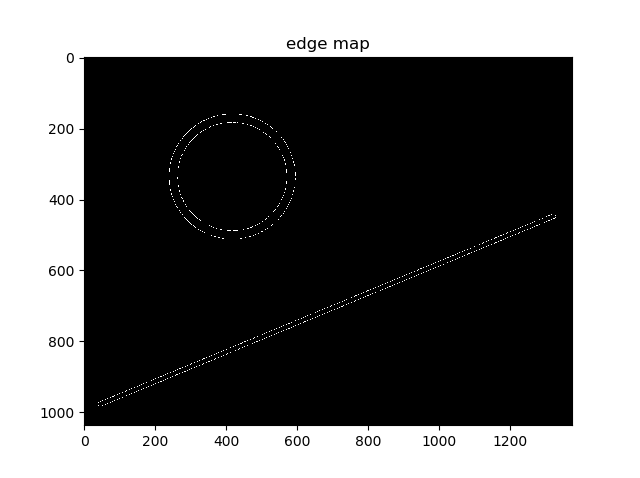
\includegraphics[width=0.95\linewidth]{pics/hw3_ex_1_synthetic_canny}
    \caption{canny of image}
  \end{subfigure}%
  \begin{subfigure}{.5\textwidth}
    \centering
    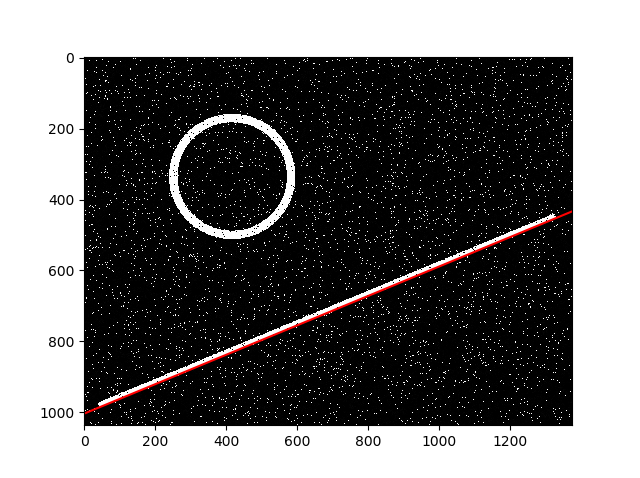
\includegraphics[width=0.95\linewidth]{pics/hw3_ex_1_synthetic_result}
    \caption{result line}
   \end{subfigure}
  \caption{Calculations of synthetic.jpg}
\end{figure}
\noindent With this low point count, it was enough to match a line. Also, the calculations were fast.
\newpage
\subsubsection{Results}
\begin{figure}[!htb]
  \vspace*{-0.5cm}
  \centering
  \begin{subfigure}{.5\textwidth}
    \centering
    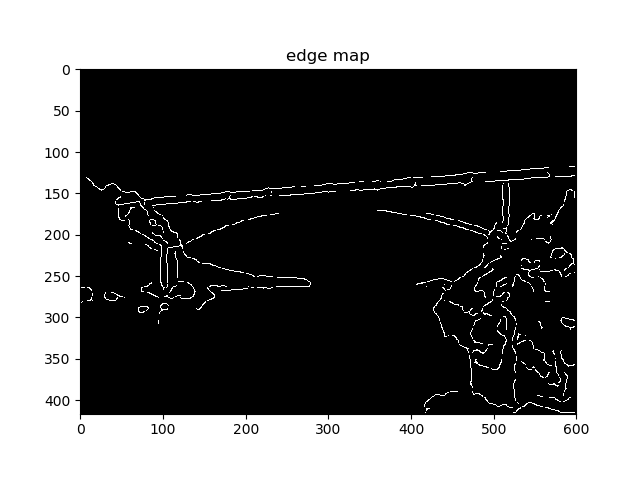
\includegraphics[width=0.7\linewidth]{pics/hw3_ex_1_bridge_canny}
    \caption{canny of image}
  \end{subfigure}%
  \begin{subfigure}{.5\textwidth}
    \centering
    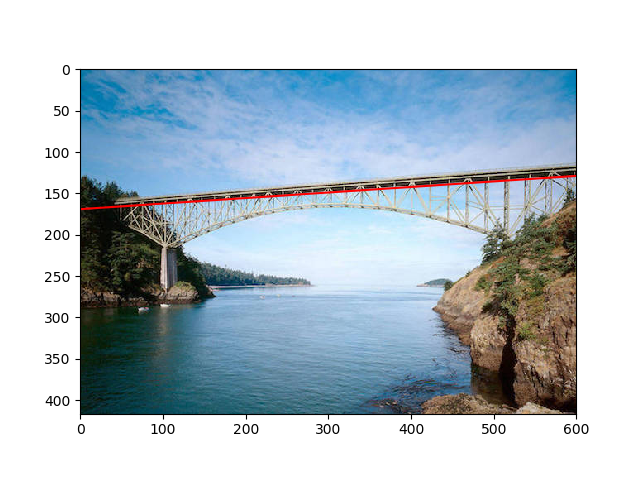
\includegraphics[width=0.7\linewidth]{pics/hw3_ex_1_bridge_result}
    \caption{result line}
   \end{subfigure}
  \caption{Calculations of bridge.jpg}
\end{figure}
\begin{figure}[!htb]
  \vspace*{-1cm}
  \centering
  \begin{subfigure}{.5\textwidth}
    \centering
    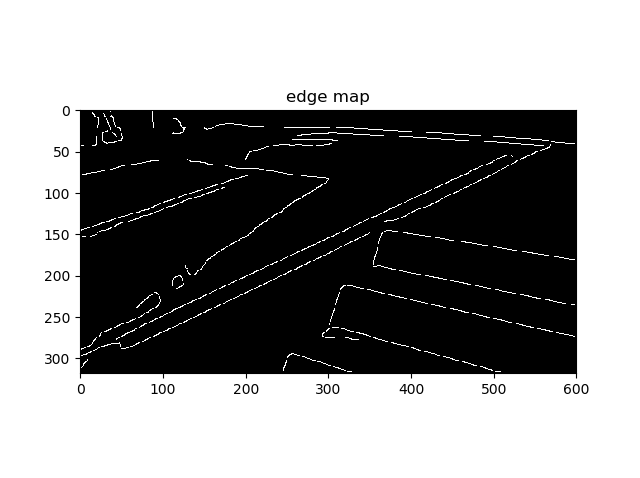
\includegraphics[width=0.7\linewidth]{pics/hw3_ex_1_pool_canny}
    \caption{canny of image}
  \end{subfigure}%
  \begin{subfigure}{.5\textwidth}
    \centering
    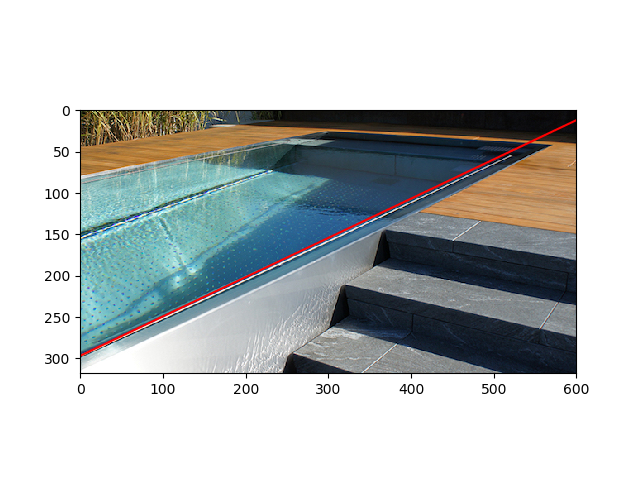
\includegraphics[width=0.7\linewidth]{pics/hw3_ex_1_pool_result}
    \caption{result line}
   \end{subfigure}
  \caption{Calculations of pool.jpg}
\end{figure}
\begin{figure}[!htb]
  \vspace*{-1cm}
  \centering
  \begin{subfigure}{.5\textwidth}
    \centering
    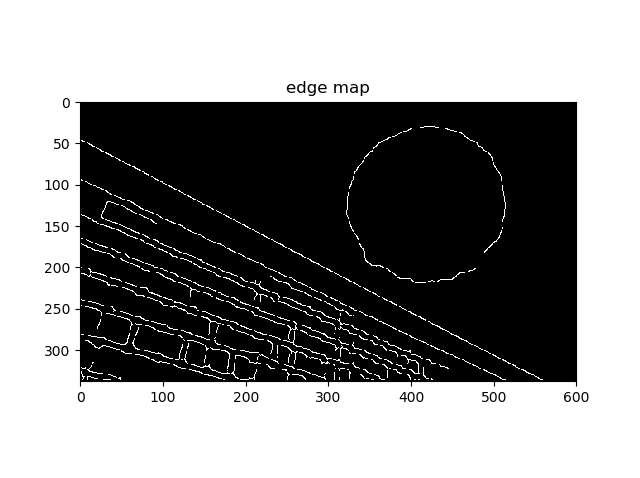
\includegraphics[width=0.7\linewidth]{pics/hw3_ex_1_tennis_canny}
    \caption{canny of image}
  \end{subfigure}%
  \begin{subfigure}{.5\textwidth}
    \centering
    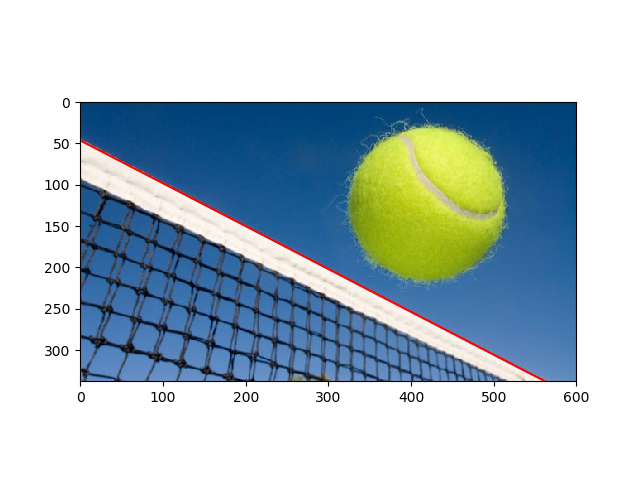
\includegraphics[width=0.7\linewidth]{pics/hw3_ex_1_tennis_result}
    \caption{result line}
   \end{subfigure}
  \caption{Calculations of tennis.jpg}
\end{figure}
\noindent It is impressing with sigma 3 resulting in a small number of points, that so an accurate solution can be achieved. RANSAC is indeed a robust method. That is also why it can be used for real-time applications, such as self-steering cars.
\newpage
\subsection{Texture Synthesis}

\subsubsection{compute\_ssd}
It is in the computation of the SSD where a performance bottleneck can be easily created. Using the build in the function of the Numpy library and using only one loop is the key to success. Also very important is the preparation of the data, as it is for the whole exercise.
\subsubsection{copy\_patch}
Implementing this function was quite easy, but better results are achieved if the mask is staying in the range from 0 - 255, even if only the min and max value existed.
\newpage
\subsubsection{Results}
\begin{figure}[!htb]
  \centering
  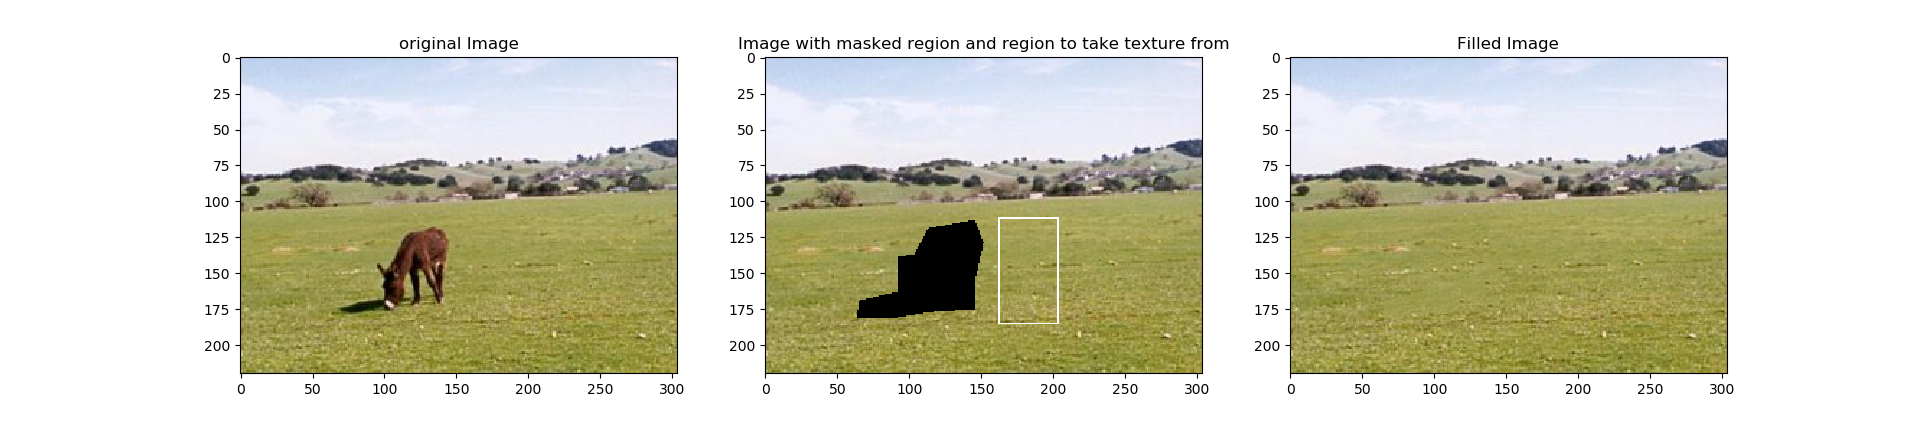
\includegraphics[width=1.0\linewidth]{pics/hw3_ex_2_donkey}
  \caption{Calculations with donkey}
\end{figure}
\begin{figure}[!htb]
  \centering
  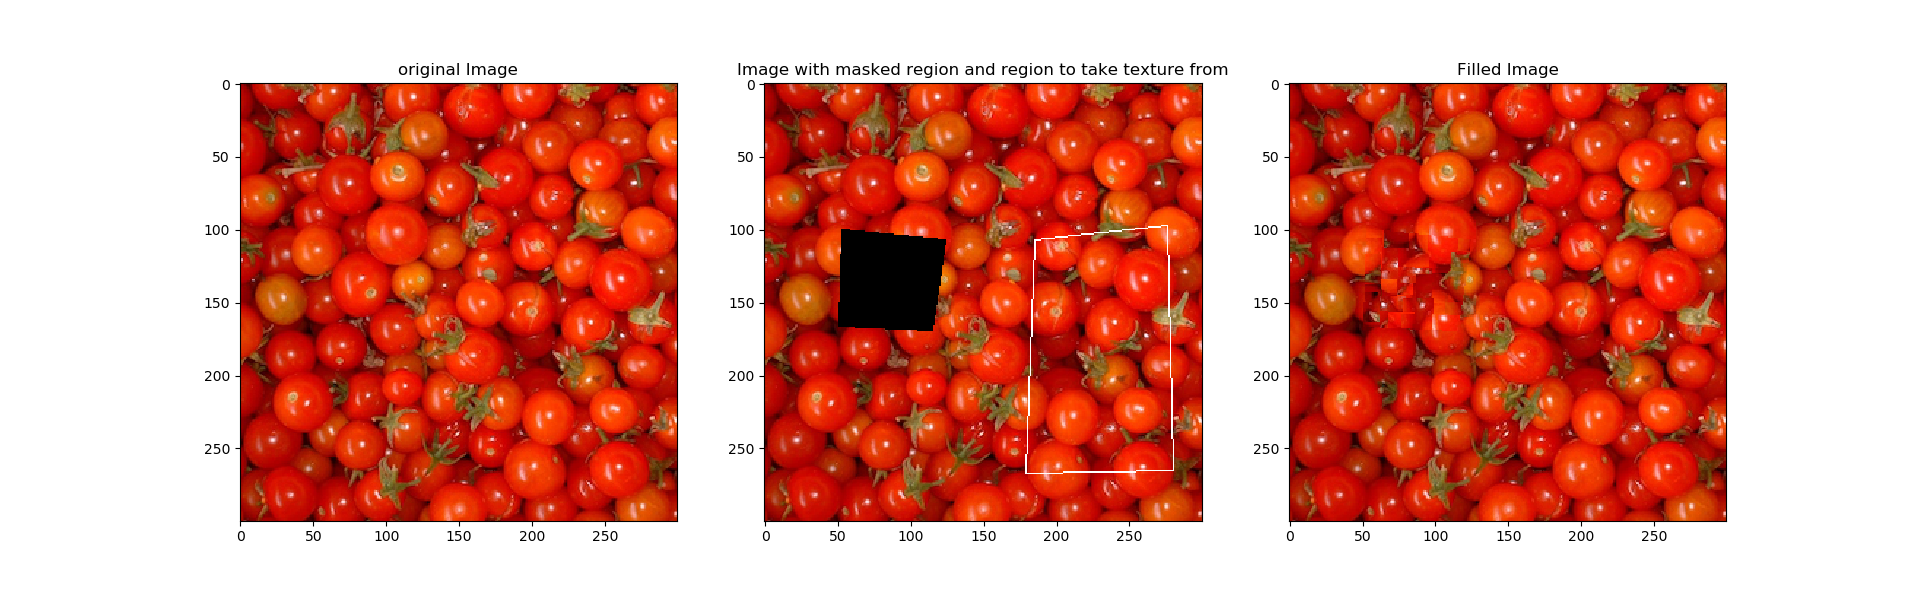
\includegraphics[width=1.0\linewidth]{pics/hw3_ex_2_tomato}
  \caption{Calculations with donkey}
\end{figure}
\begin{figure}[!htb]
  \centering
  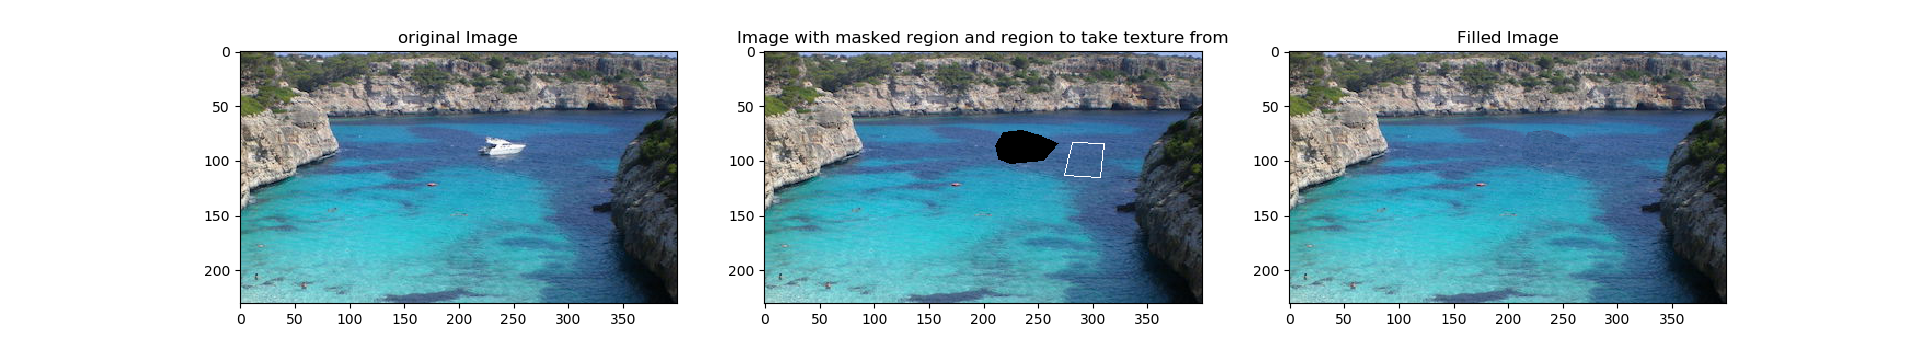
\includegraphics[width=1.0\linewidth]{pics/hw3_ex_2_yacht}
  \caption{Calculations with donkey}
\end{figure}
\noindent Changing the half patch size variable to 5 and 10 did not really help to achieve better results. However, choosing the best texture patch is based on a random gauss, so the image looks from calculation to calculation a bit better or worse. With simple textures with less detail, the results are amazingly good. Several optimizations could be made in the choosing of the textures samples for the empty spot in the image.
\newpage
\subsection{Conclusion}
The work in this assignment was demanding and made a lot of fun. Only if everything is comprehended a solution could be rudimentary created. Lot of work was made in the preparation of the incoming data for the right structures for the calculations.


\begin{thebibliography}{1}
  \bibitem{comp_intro} 
  Alasdair McAndrew
  \\\textit{A Computational Introduction to Digital Image Processing (2015)}. (English)  
  \bibitem{IEEE} 
  Alexei A Efros and Thomas K Leung.
  \\\textit{Texture synthesis by non-parametric sampling. In Computer Vision 1999. The Proceedings of the Seventh IEEE International Conference on, volume 2, pages 10331038. IEEE, 1999}. (English)
  \bibitem{RANSAC} 
  Random sample consensus
  \\\textit{https://en.wikipedia.org/wiki/Random\_sample\_consensus (2019)}. (English)  
\end{thebibliography}


\end{document}
